\chapter{基于联邦半监督学习的样本参与方生成方法}
\thispagestyle{others}
\pagestyle{others}
\xiaosi

\section{本章引言}
联邦学习使多个参与方能够在不暴露私有数据的情况下协作构建机器学习模型。特别是,纵向联邦学习(VFL)利用对齐样本的分布式特征来构建联合模型。然而,VFL要求参与方共享足够大的对齐样本集——这一假设在实践中常常不成立,因为只有一小部分数据是对齐的,留下大部分未对齐的数据未被利用。

受第3章讨论的局限性启发,本章
FPU-Multitask-Synthesis(VFPU-M-Syn),一种基于纵向联邦半监督学习的样本生成方法,旨在在对齐样本有限时提升VFL性能。具体而言,VFPU-M-Syn估计缺失特征的表示。对于高度相关的特征,VFPU-M-Syn预测未标记样本的伪标签以扩展训练集;而对于相关性较低的特征,则采用生成模型合成数据。随后,VFPU-M-Syn在这些增强的数据视图上联合训练三个分类器,以提高整体VFL模型的性能。此外,VFPU-M-Syn通过确保参与方之间不交换原始数据或模型参数来保护数据隐私,满足联邦学习环境中的关键要求。

本章的结构安排如下:3.2 节将对问题进行分析定义,3.3节将系统性地阐述基于半监督学习的纵向联邦参与方样本生成方法框架,并详细介绍 VFPU-M-Syn 的执行流程和算法设计。3.3 节在多个真实数据集上进行实验,验证 VFPU 方法的有效性,并对实验结果进行深入分析。最后,3.4 节对本章的研究工作进行总结。

\section{问题分析与定义}
考虑一个典型的两方纵向联邦学习(Vertical Federated Learning, VFL)场景,其中涉及两个参与方通过各自独立的特征集进行合作学习,在保证数据隐私和安全的前提下,共同训练一个机器学习模型\textsuperscript{\cite{yang2019federated}}。参与方包括 Party A 和 Party B,其中只有一方拥有标签。首先,Party A 拥有数据集:
\begin{equation}
	\mathcal{D}^A := \{X^A_i\}_{i=1}^{n^A}
\end{equation}
其中,$X^A_i$ 是第 $i$ 个样本的特征向量,$n^A$ 是样本数量。Party A 的数据仅包含特征,不包含标签。接着,Party B 拥有数据集:
\begin{equation}
	\mathcal{D}^B := \{(X^B_i, Y^B_i)\}_{i=1}^{n^B}
\end{equation}
其中,$X^B_i$ 是第 $i$ 个样本的特征向量,$Y^B_i \in \{0,1\}^C$ 是对应的独热编码(one-hot encoding)真实标签,$C$ 表示类别数,$n^B$ 是样本数量。Party B 拥有标签,这在 VFL 中至关重要,因为标签通常用于监督学习任务。然而,Party B 缺乏足够的特征来单独构建一个准确的模型,因此需要利用 Party A 提供的补充特征,如图 \ref{fig:Missing}\subref{MissingTwo} 所示。
%调整图片与上方文字之间的间距
\vspace{-0.1cm}
\begin{figure}[!h]
	\centering
	\subfigure[]{
		\label{MissingOne}
		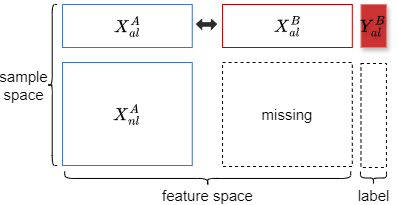
\includegraphics[width=0.45\textwidth]{chapters/imgs/MissingOne}}
	\hspace{0.01\textwidth}  % 适当增加间距
	\subfigure[]{
		\label{MissingTwo}
		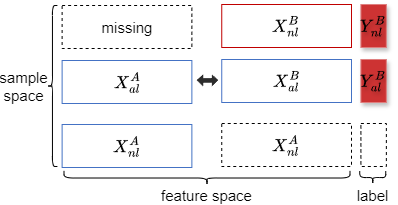
\includegraphics[width=0.45\textwidth]{chapters/imgs/MissingTwo}}
	
	\bicaption[\xiaosi \songti 纵向联邦样本未对齐缺失情况]%
	{\centering \wuhao 纵向联邦样本未对齐缺失情况。(a) B 方缺失情况;(b) 双方缺失情况}%
	{\centering \wuhao Vertical Federated Learning with Unaligned Samples. (a) Missing data in party B; (b) Missing data in both parties}    
	\label{fig:Missing}
\end{figure}
%调整图片与下方文字之间的间距
\vspace{-0.35cm}

需要强调的是,$\mathcal{D}^A$ 和 $\mathcal{D}^B$ 分别由 Party A 和 Party B 私有保存,双方不能互相暴露其数据集。

在 VFL 中,Party A 和 Party B 的数据集 $\mathcal{D}^A$ 和 $\mathcal{D}^B$ 包含了不同样本的特征。为了进行联合学习,需要将具有相同身份的样本对齐。假设通过隐私保护的加密实体匹配技术,双方已经完成了样本对齐,得到了对齐样本集:
\begin{equation}
	\mathcal{D}_{al} := \{X^A_{i_{al}}, X^B_{i_{al}}, Y^B_{i_{al}}\}_{i=1}^{n_{al}}
\end{equation}
其中,$n_{al}$ 是对 齐样本的数量。Party A 拥有对齐样本的特征:
\begin{equation}
	\mathcal{D}^A_{al} := \{X^A_{i_{al}}\}_{i=1}^{n_{al}}
\end{equation}
Party B 拥有对齐样本的特征和标签:
\begin{equation}
	\mathcal{D}^B_{al} := \{X^B_{i_{al}}, Y^B_{i_{al}}\}_{i=1}^{n_{al}}
\end{equation}
如果将 $\mathcal{D}^A$ 和 $\mathcal{D}^B$ 连接起来,并使具有相同身份的样本对齐,我们将得到一个如图 \ref{fig:Missing}\subref{MissingTwo} 所示的单一数据集。这个数据集是垂直分割的,每个方拥有该数据集的一个垂直分区(或部分视图),这正是“纵向联邦学习”一词的由来。然而,两方之间通常只存在有限数量的对齐样本。除了对齐样本外,每个方还拥有一些非对齐样本,即没有来自另一方对应样本的数据。对于 Party A,非对齐样本表示为:
\begin{equation}
	\mathcal{D}^A_{nl} := \{X^A_{i_{nl}}\}_{i=1}^{n^A_{nl}}
\end{equation}
对于 Party B,非对齐样本表示为:
\begin{equation}
	\mathcal{D}^B_{nl} := \{X^B_{i_{nl}}, Y^B_{i_{nl}}\}_{i=1}^{n^B_{nl}}
\end{equation}
从单一表格数据集(见图 \ref{fig:Missing}\subref{MissingTwo})的角度来看,每个方对于另一方的非对齐样本都没有对应的特征(或标签)。我们将这些特征(或标签)视为“缺失”。图 \ref{fig:Missing}\subref{MissingTwo} 中的各方样本未对齐的情况可以划分为两个图 \ref{fig:Missing}\subref{MissingOne} 所示的情况,对于B方缺失和对于A方缺失。所以,只需解决其中一个问题即可。

传统的 VFL 方法仅使用对齐样本 $\mathcal{D}_{al}$ 来构建联邦机器学习模型,而将非对齐样本 $\mathcal{D}^A_{nl}$ 和 $\mathcal{D}^B_{nl}$ 弃置不用。这种做法在对齐样本数量较少时,可能会限制模型的性能,因为大量潜在有用的数据被忽略。

本章提出了一种新的方法 VFPU-M-Syn,旨在充分利用非对齐样本 $\mathcal{D}^A_{nl}$ 和 $\mathcal{D}^B_{nl}$,以提升纵向联邦学习(VFL)模型的性能。该方法结合了 纵向联邦半监督学习 和 表格数据生成技术,通过将对齐样本 $\mathcal{D}_{al}$ 视为有标签数据(其中 $X^A_{al}$ 的“标签”可看作 $X^B_{al}$ 的特征值),而将非对齐样本 $\mathcal{D}^A_{nl}$ 视为无标签数据,利用半监督学习从对齐样本中学习以增强模型的泛化能力,同时采用表格数据生成技术填补与 Party A 相关性较弱的特征缺失值,并与纵向联邦学习相结合优化数据补全。相比传统 VFL 方法,VFPU-M-Syn 不仅利用了对齐样本 $\mathcal{D}_{al}$,还充分利用了非对齐样本 $\mathcal{D}^A_{nl}$ 和 $\mathcal{D}^B_{nl}$,显著提高了数据利用率;通过纵向联邦半监督学习,模型能从无标签数据中提取有用信息,进一步提升泛化能力;而表格数据生成技术的引入则使得缺失特征的填补更加合理,从而优化了数据填补策略并提高了模型整体性能。总之,VFPU-M-Syn 在传统 VFL 框架基础上引入创新技术,充分利用非对齐样本,在对齐样本有限的情况下显著提升了 VFL 模型的准确性和泛化能力。
\section{基于半监督学习的纵向联邦参与方样本生成方法方法框架}
如图 \ref{fig:VFPU-M-Syn} 所示,VFPU-M-Syn 方法的核心包含三个主要流程,这三个流程共同协作以实现跨方数据的高效处理和特征生成。首先,在 Process I 中,算法通过计算跨方特征之间的相关性,评估和量化各个特征之间的相互依赖关系。这一过程的目标是确保在纵向联邦学习框架中,不同方的特征能够高效对齐,并通过特征相关性分析揭示不同数据源之间可能存在的潜在依赖结构,从而为后续的建模步骤提供更加精确和有针对性的特征信息。接下来,在 Process II 中,方法采用纵向联邦半监督学习算法来进行数据预测。在这一阶段,算法通过结合来自多个方的信息,并利用半监督学习的策略,有效地预测出缺失或未标记的数据。这一过程不仅保证了数据的完整性,还通过有效利用部分标记数据和大量未标记数据,增强了模型的预测能力和鲁棒性。通过这种方式,VFPU-M-Syn 方法能够在数据不完全或部分缺失的情况下,依然保持较高的预测精度。最后,在 Process III 中,VFPU-M-Syn 方法利用生成模型生成数据。通过对已预测数据和其他相关特征的建模,生成模型能够创造出与真实数据相似的合成数据。这些生成的数据不仅能够补充现有数据的不足,还可以用来进一步优化模型的训练过程,提升模型在实际应用中的泛化能力。生成的数据也有助于应对训练数据中可能出现的偏差或不均衡问题,进一步增强模型的稳定性和可靠性。下面的小节我将分别介绍这三个流程。

%调整图片与上方文字之间的间距
\vspace{-0.1cm}
\begin{figure}[H]  % 创建一个浮动图形环境,[h]表示尽量将图片放在当前位置(here)
	\centering     % 使图片居中显示
	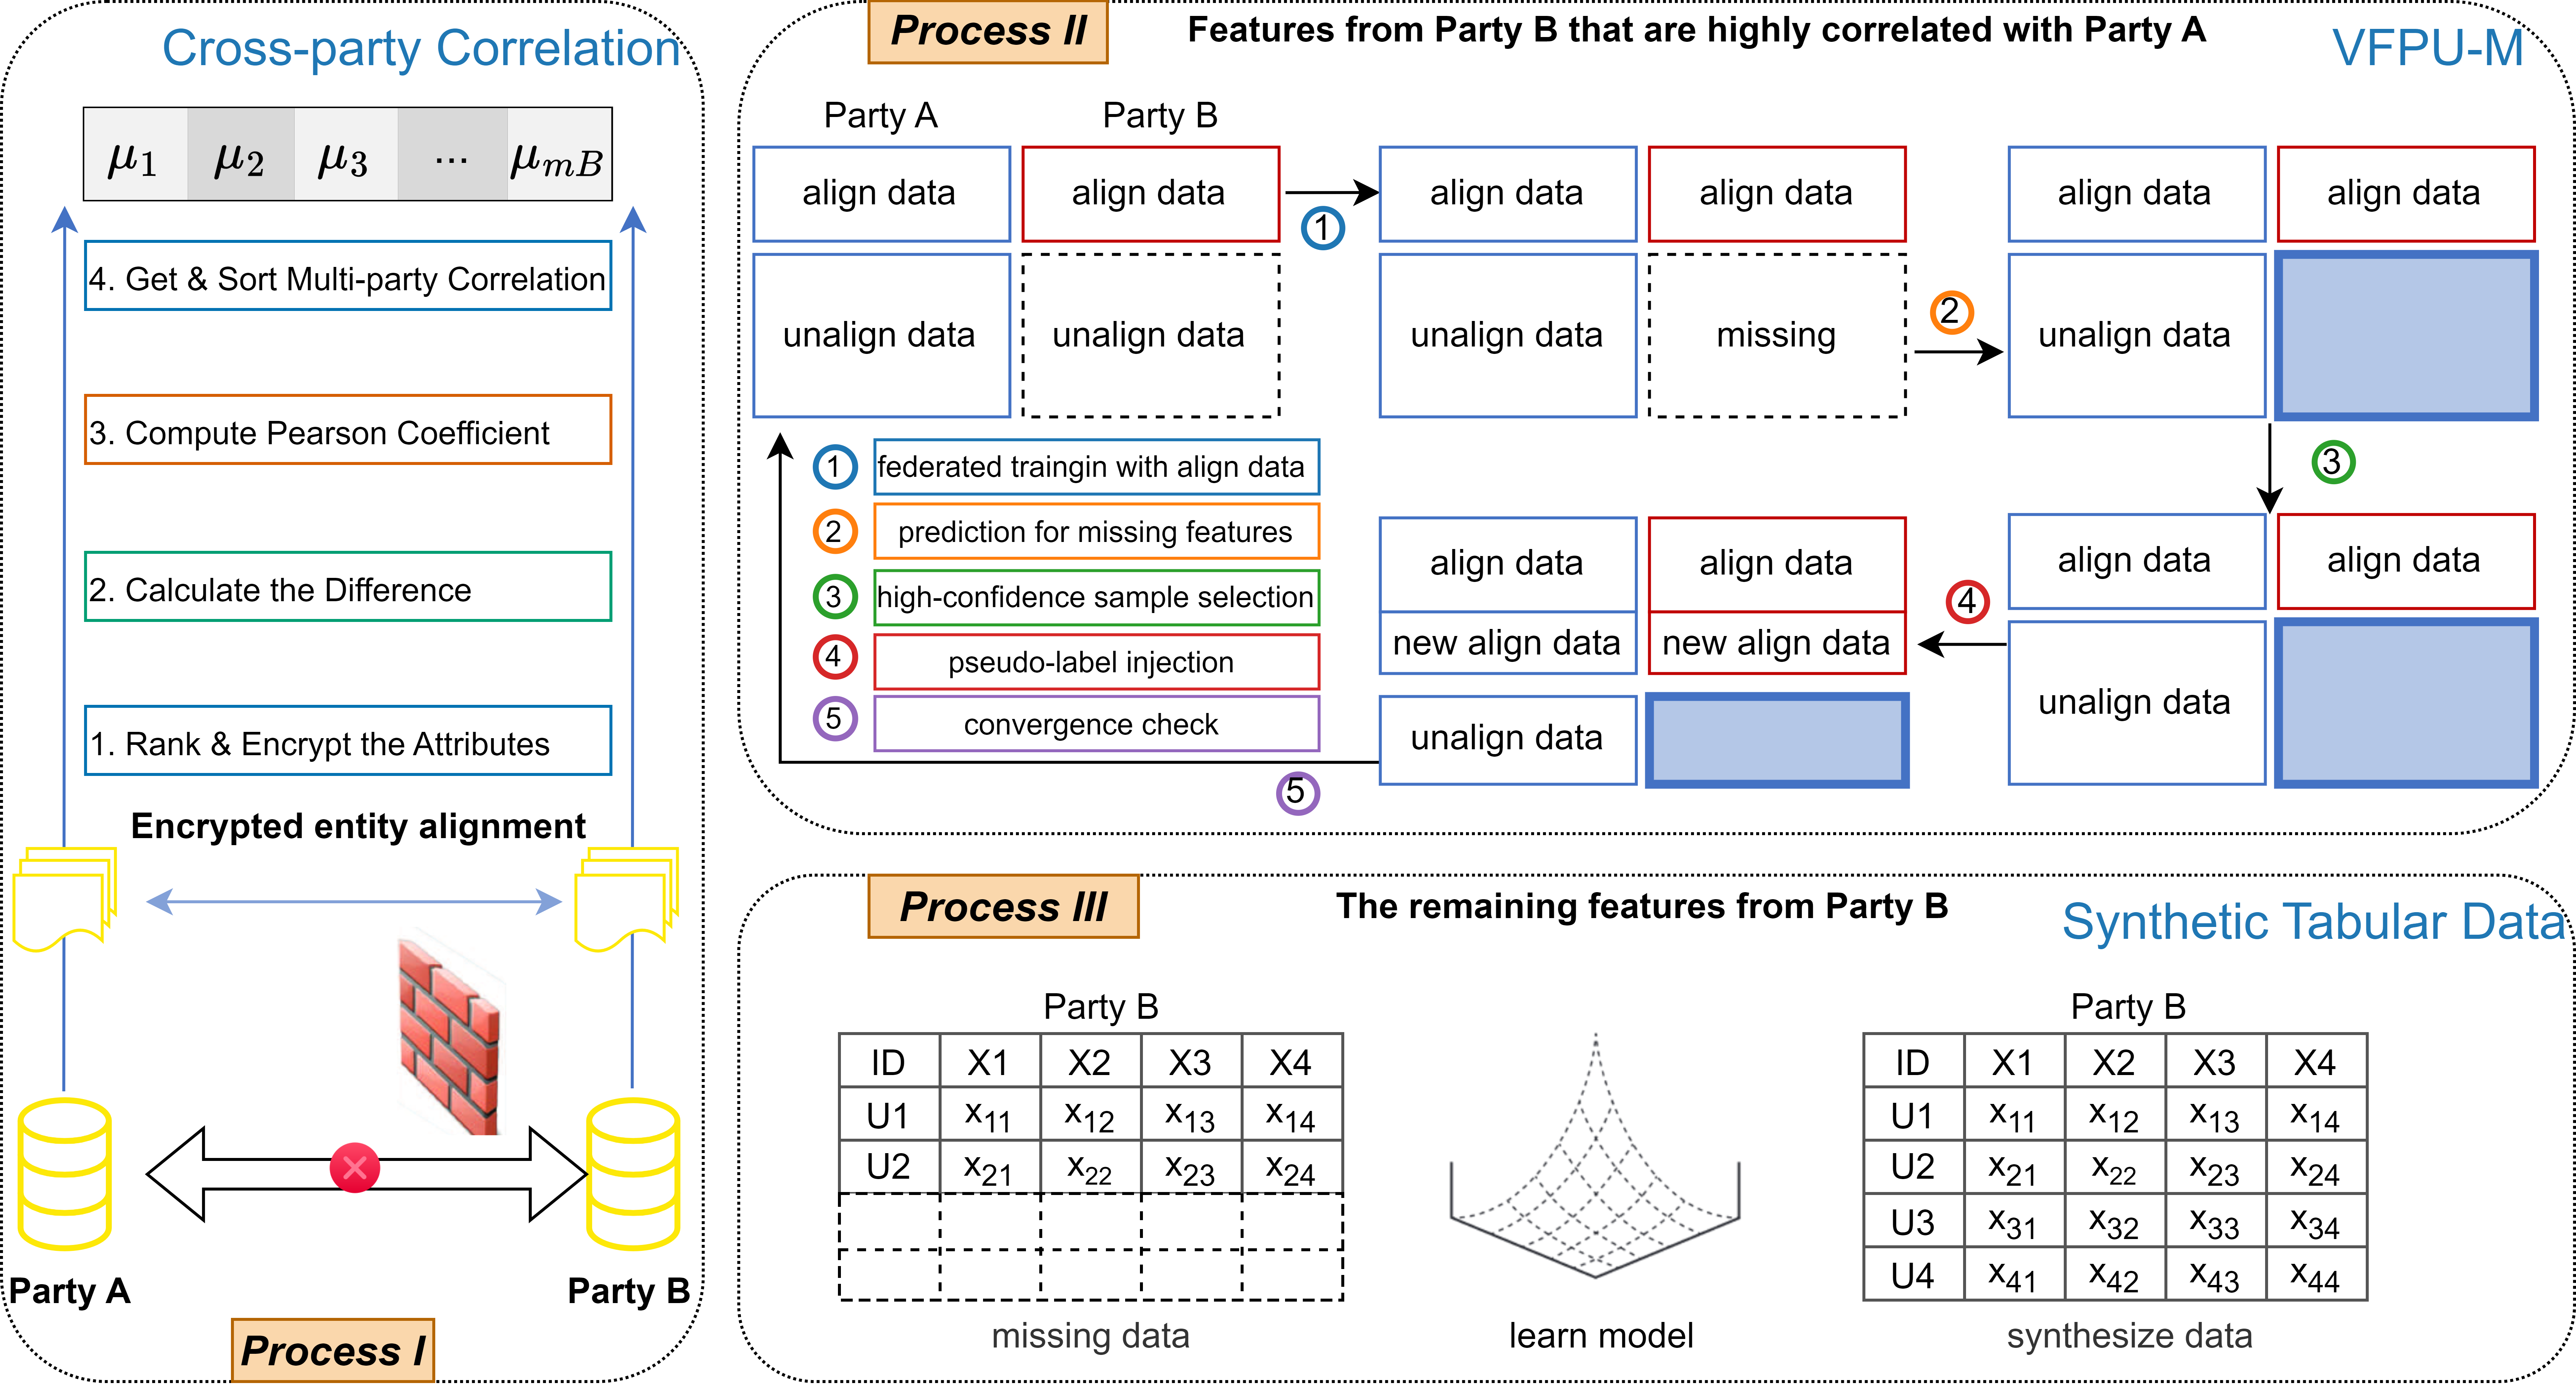
\includegraphics[width=0.9\textwidth]{chapters/imgs/VFPU-M-Syn}  
	% 插入图片,宽度设为页面宽度的90%,图片路径为chapters/imgs/Figure 1 in JEPG format
	
	\bicaption[\xiaosi VFPU-M-Syn算法总体流程]{\wuhao VFPU-M-Syn算法总体流程}{\wuhao The overall process of the proposed VFPU-M-Syn algorithm}
	% 使用bicaption命令创建双语标题
	% [\xiaosi VFPU算法总体流程] - 目录中显示的标题,使用小四号字体
	% {\wuhao VFPU算法总体流程} - 中文标题,使用五号字体
	% {\wuhao The overall process...} - 英文标题,使用五号字体
	
	\label{fig:VFPU-M-Syn}  % 为图片设置标签,可以在文中使用\ref{fig:VFPU}引用此图
\end{figure}
%调整图片与下方文字之间的间距
\vspace{-0.35cm}

\subsection{计算跨方特征相关性}
在纵向联邦学习(Vertical Federated Learning, VFL)框架中,不同参与方(Parties)拥有相同样本但不同特征的异构数据。为了有效利用对齐样本的特征信息,需要量化跨参与方特征之间的统计关联性。本节提出了一种基于隐私保护的Spearman秩相关分析方法,用于构建跨方特征相关性排序体系。

设协调方(Coordinator)$ C $ 作为可信第三方,负责生成同态加密(Homomorphic Encryption, HE)密钥对 $ \{\text{pk}, \text{sk}\} $,其中:
- $ \text{pk} $ 为公钥(Public Key),用于加密数据;
- $ \text{sk} $ 为私钥(Secret Key),用于解密数据。

协调方 $ C $ 将公钥 $ \text{pk} $ 分发给参与方 A(Party A)和参与方 B(Party B),以便它们对数据进行加密计算,而不直接暴露原始数据,具体计算流程如下:

定义 1 特征列秩向量:设参与方 A 的特征空间为 $ \Phi^A = \{\varphi^A_1, \varphi^A_2, ..., \varphi^A_{m_A}\} $,$ m_A $ 表示 A 方的特征维数,即 A 方拥有 $ m_A $ 个特征。$ \varphi^A_p \in \mathbbm{R}^{n_{al}} $ 表示 A 方第 $ p $ 个特征在对齐样本集 $ \mathcal{D}^A_{al} $ 上的观测向量,$ \varphi^A_p = [\varphi^A_{p1}, \varphi^A_{p2}, ..., \varphi^A_{pn_{al}}] $ 表示该特征在所有对齐样本上的取值,$ n_{al} $ 为对齐样本的数量。

同理,参与方 B 的特征空间为 $ \Phi^B = \{\varphi^B_1, \varphi^B_2, ..., \varphi^B_{m_B}\} $,$ m_B $ 表示 B 方的特征维数,即 B 方拥有 $ m_B $ 个特征。$ \varphi^B_q \in \mathbbm{R}^{n_{al}} $ 表示 B 方第 $ q $ 个特征在对齐样本集 $ \mathcal{D}^B_{al} $上的观测向量。$ \varphi^B_q = [\varphi^B_{q1}, \varphi^B_{q2}, ..., \varphi^B_{qn_{al}}] $ 表示该特征在所有对齐样本上的取值,$ n_{al} $ 为对齐样本的数量。

对于任意特征列 $ \varphi^A_p $,计算其秩向量(Rank Vector):
\begin{equation}
	R^A_p = [r^A_{p1}, r^A_{p2}, ..., r^A_{pn_{al}}]
\end{equation}
$ r^A_{pi} $ 表示样本 $ i $ 在特征 $ \varphi^A_p $ 上的秩次(Rank),即该样本在该特征列中的排序位置,若存在相同值,则采用平均秩(Average Rank)处理。类似地,B 方的特征列 $ \varphi^B_q $ 也可以计算出对应的秩向量:
\begin{equation}
	R^B_q = [r^B_{q1}, r^B_{q2}, ..., r^B_{qn_{al}}]
\end{equation}

步骤 1 加密秩传输:A 方 使用公钥 $ \text{pk} $ 对秩向量 $ R^A_p $ 进行同态加密,得到:
\begin{equation}
	[R^A_p] = \{\text{Enc}(r^A_{p1}), \text{Enc}(r^A_{p2}), ..., \text{Enc}(r^A_{pn_{al}})\}
\end{equation}
并将加密后的秩向量发送给 B 方。类似地,B 方 也对自己的秩向量 $ R^B_q $ 进行同态加密,得到:
\begin{equation}
	[R^B_q] = \{\text{Enc}(r^B_{q1}), \text{Enc}(r^B_{q2}), ..., \text{Enc}(r^B_{qn_{al}})\}
\end{equation}

步骤 2 秩差计算:对于任意特征对 $ (f^A_p, f^B_q) $,B 方计算加密秩差向量:
\begin{equation}
	[D_{pq}] = \left[ \text{Enc}(r^A_{p1} - r^B_{q1}), ..., \text{Enc}(r^A_{pn_{al}} - r^B_{qn_{al}}) \right]
\end{equation}
其中,$ d_{pq}^i = r^A_{pi} - r^B_{qi} $ 表示样本 $ i $ 在 A 方特征 $ f^A_p $ 和 B 方特征 $ f^B_q $ 上的秩次之差,由于同态加密支持加法运算,B 方可以在加密状态下直接计算秩差,而无需解密。B 方将加密秩差向量 $ [D_{pq}] $ 发送给协调方 $ C $。

步骤 3 Spearman相关性计算:协调方 $ C $ 解密 $ [D_{pq}] $,得到:
\begin{equation}
	d_{pq}^i = r^A_{pi} - r^B_{qi}, \quad i = 1, ..., n_{al}
\end{equation}
然后计算 Spearman 相关系数:
\begin{equation}
	\rho_{pq} = 1 - \frac{6\sum_{i=1}^{n_{al}} (d_{pq}^i)^2}{n_{al}(n_{al}^2 - 1)}
\end{equation}
$ \rho_{pq} $ 表示 A 方特征 $ f^A_p $ 与 B 方特征 $ f^B_q $ 之间的 Spearman 相关系数。最终,构建跨方相关性矩阵:
\begin{equation}
	\mathbf{M} \in \mathbbm{R}^{m_A \times m_B}, \quad \mathbf{M}(p,q) = \rho_{pq}
\end{equation}
$ \mathbf{M}(p,q) $ 存储 A 方第 $ p $ 个特征列与 B 方第 $ q $ 个特征列的 Spearman 相关系数。

定义 2 特征关联强度:对于 B 方的每个特征 $ f^B_q $,计算其与 A 方所有特征的平均关联强度:
\begin{equation}
	\mu_q = \frac{1}{m_A} \sum_{p=1}^{m_A} \rho_{pq}, \quad q=1,...,m_B
\end{equation}
$ \mu_q $ 表示 B 方特征 $ f^B_q $ 对 A 方特征空间的综合依赖程度。

步骤 4 生成排序列表:构建特征重要性序列:
\begin{equation}
	\mathcal{L}_B = \{(\mu_q, f^B_q)\}_{q=1}^{m_B}
\end{equation}
按 $ \mu_q $ 降序排列,得到排序后的特征列表
\begin{equation}
	\mathcal{L}_B^{sorted}
\end{equation}
该列表用于指导利用联邦半监督学习对 B 方对齐样本的特征补全,优先使用联邦半监督学习方法补充与 A 方特征关联性强的维度。
\subsection{纵向联邦半监督方法预测数据}
如图 \ref{fig:VFPU-M-Syn} 所示,在计算跨方相关性列表之后,研究进入 Process II 阶段。在该阶段,我们从 B 方 中选择一部分与 A 方 具有较高相关性的列,以此作为生成过程的基础。具体而言,该选择过程基于前一阶段计算得到的跨方相关性列表,确保所选列能够最大程度地保留和反映 A 方 的特征信息,从而提高后续生成过程的准确性和有效性。在 Process II 阶段,列的选择标准通常依赖于相关性阈值设定,即仅保留那些与 A 方 相关性超过某一特定阈值的列。

在这一过程中,本方法将B方的高相关性特征逐列拆分,每一列特征单独作为一个标签列。随后,A方的数据与基于纵向联邦半监督学习方法生成的B方部分数据共同构成训练数据集,从而形成一个典型的纵向联邦半监督学习框架[1]。如图所示,$X^A$ 表示A方的数据,而 ${{X}^{{{B}_{predict}}}}$ 代表通过纵向联邦半监督学习方法推测得到的B方部分数据。此外,$f_{q}^{B}$ 表示B方的第 $q$ 个特征列,在本方法中,该特征列被视为 $X^A$ 和 ${{X}^{{{B}_{predict}}}}$ 进行纵向联邦学习时的标签。

在该框架下,A方和B方的数据仍然保持隐私保护,即A方无法直接访问B方的原始数据,B方也无法直接获取A方的数据。然而,通过联邦学习的协作训练机制,A方可以利用自身数据和部分推测得到的B方数据进行模型训练,以优化对B方特征的预测能力。与此同时,B方的高相关性特征被逐列拆分,使得每一列特征都可以单独作为监督信号,从而有效地提升模型的学习能力。

在本研究中,该问题被重新表述为一个纵向联邦半监督学习(Vertical Federated Semi-Supervised Learning, VFSSL)问题,其中特征集 $X^A$ 和 $X^{B_{\text{predict}}}$ 的数据被划分为有标签部分和无标签部分。Liu等人\textsuperscript{\cite{liu2023multi}}提出了VFPU(Vertical Federated Positive-Unlabeled Learning)算法来解决纵向联邦半监督学习问题。然而,VFPU 方法主要适用于PU(Positive-Unlabeled)学习,即仅包含正样本和未标记样本的情况,而在本研究中,$ f_q^B $ 特征列可能涉及二分类、多分类甚至回归任务,VFPU 方法无法直接适用。因此,本文在 VFPU 方法的基础上进行了改进,提出了一种新的方法——VFPU-M(Multi-task VFPU),使其能够适用于多种任务类型。VFPU-M 主要通过以下五个步骤实现纵向联邦半监督学习,如图 \ref{fig:VFPU-M-Syn} 所示。
\begin{enumerate}
	\item 基于对齐数据进行纵向联邦训练  
	\item 利用训练好的基学习器对未对齐数据进行预测  
	\item 计算预测结果的置信度  
	\item 选择高置信度样本加入对齐数据集  
	\item 重复上述过程,直至满足终止条件  
\end{enumerate}
通过 VFPU-M 方法,本研究能够在纵向联邦学习框架下有效利用无标签数据,从而提升模型的泛化能力,并适用于多种任务类型(如二分类、多分类和回归任务)。实验结果表明,VFPU-M 在不同任务场景下均能取得优于传统 VFPU 方法的性能,进一步验证了其有效性和适用性。

在本阶段的研究工作中,主要需要执行两个核心算法,以确保数据处理和模型训练的有效性。这两个算法分别为:算法1——基于纵向联邦半监督学习(Vertical Federated Semi-Supervised Learning, VFSSL)的方法用于数据生成的过程,以及算法2——VFPU-M(Vertical Federated PU Learning with Model Adaptation)算法。在后续章节中,我们将对这两个算法的理论基础、实现细节及其在本研究中的具体应用进行详细介绍。

(1) 算法 1:基于纵向联邦半监督学习的数据生成过程

本小节介绍了一种基于纵向联邦半监督学习(Vertical Federated Semi-supervised Learning, VFSL)的方法,用于生成 B 方缺失的数据。该方法的核心思想是利用 A 方与 B 方对齐数据之间的统计相关性,结合联邦学习框架,在保证数据隐私的前提下,对 B 方未对齐样本进行特征补全。算法 4-1 详细描述了该数据生成过程。

\vspace{-0.2cm} 
\begin{table}[H]
	\centering
	\renewcommand{\arraystretch}{1.0}
	{\songti \wuhao
	\begin{tabular}{p{13.2cm}}
		\toprule[1.5pt]
		\makecell[l]{\songti\wuhao  算法 4-1 纵向联邦半监督方法生成数据过程}\\
		\midrule[0.75pt]
		\makecell[l]{\wuhao \textbf{输入:} A方对齐数据集 $X_{al}^A$, 未标记数据集 $X_{nl}^A$,B 方特性相关性列表 $\mathcal{L}_B$}\\
		\makecell[l]{\wuhao \quad 对齐数据集样本数量 $n_{al}$,标记数据集的样本数量 $n_{nl}$,相关性阈值 $\tau$}\\
		\makecell[l]{\wuhao \textbf{输出:} $X^{B_{predict}}$: 最终通过预测方法生成的B方数据}\\
		\makecell[l]{\wuhao \textbf{Process:}}\\
		\makecell[l]{\wuhao 1: Initialize $X^{B_{predict}} = \emptyset$, $\mathcal{L}_B^{\text{predict}} = \{(\mu_q, \phi^B_q) \in \mathcal{L}_B \mid u_q > \tau\}$}\\
		\makecell[l]{\wuhao 2: \textbf{for} $(\mu_q, \phi^B_q) \in \mathcal{L}_B^{\text{predict}}$ \textbf{do}}\\
		\makecell[l]{\wuhao 3: \quad $X_{al}^{B_{predict}} = \{x_{i}^{B_{predict}}\}_{i=1}^{n_{al}}$}\\
		\makecell[l]{\wuhao 4: \quad $X_{nl}^{B_{predict}} = \{x_{i}^{B_{predict}}\}_{i=n_{al}+1}^{n_{al}+n_{nl}}$}\\
		\makecell[l]{\wuhao 5: \quad $p = \text{VFPU-M}(X_{al}^A, X_{nl}^A, X_{al}^{B_{predict}}, X_{nl}^{B_{predict}}, \phi^B_q)$}\\
		\makecell[l]{\wuhao 6: \quad $X^{B_{predict}} = X^{B_{predict}} \cup \{p\}$}\\
		\makecell[l]{\wuhao 7: \textbf{end for}}\\
		\makecell[l]{\wuhao 8: 得到 $X^{B_{predict}}$}\\
		\bottomrule[1.5pt]
	\end{tabular}
}
	\label{tab:algo-vfpu}
\end{table}
\vspace{-0.56cm}
算法的输入包括以下几个关键元素:A 方对齐数据:$X_{al}^A \in \mathbbm{R}^{n_{al} \times d_A}$,表示 A 方与 B 方样本空间对齐的特征矩阵,其中 $n_{al}$ 为对齐样本的数量,$d_A$ 为 A 方特征维度。A 方未对齐数据:$X_{nl}^A \in \mathbbm{R}^{n_{nl} \times d_A}$,表示 A 方未对齐部分的特征矩阵,其中 $n_{nl}$ 为未对齐样本的数量。B 方相关系数列表:$\mathcal{L}_B = \{(\mu_q, \phi^B_q)\}_{q=1}^{d_B}$,其中 $\mu_q$ 表示 B 方特征列 $\phi^B_q$ 与 A 方数据的皮尔逊相关系数,$d_B$ 为 B 方特征维度。相关性阈值:$\tau$,用于筛选与 A 方数据具有显著相关性的 B 方特征列。该阈值的选取通常基于统计显著性检验,以确保筛选出的特征在统计上具有可靠性。

算法的核心目标是利用 A 方数据预测 B 方未对齐样本的特征值,并生成完整的 B 方数据矩阵 $X^{B_{predict}}$。整个过程可分为以下三个主要步骤:

初始化阶段:目标数据集 $X^{B_{predict}}$ 为空集,表示尚未生成任何 B 方数据。通过相关性筛选,从 $\mathcal{L}_B$ 中选取所有相关性系数大于阈值 $\tau$ 的特征列,构造预测特征集合:
\begin{equation}
	\mathcal{L}_B^{\text{predict}} = \{(\mu_q, \phi^B_q) \in \mathcal{L}_B \mid \mu_q > \tau\}
\end{equation}
该筛选过程通常采用假设检验方法,以确保仅保留统计上显著相关的特征,从而提高数据生成的可靠性。特征级联邦数据生成:对于每个满足相关性筛选条件的特征列 $(\mu_q, \phi^B_q) \in \mathcal{L}_B^{\text{predict}}$,执行以下步骤,数据分区  将 B 方特征列 $\phi^B_q$ 的预测数据划分为:对齐部分:$X_{al}^{B_{predict}} \in \mathbbm{R}^{n_{al}}$,对应于 A 方对齐样本的 B 方特征值。未对齐部分:$X_{nl}^{B_{predict}} \in \mathbbm{R}^{n_{nl}}$,需要通过联邦学习方法进行预测。这种数据分区方式与 A 方数据结构保持一致,有助于后续联邦建模的执行。联邦预测建模:采用 VFPU-M(Vertical Federated Prediction with Unlabeled Missing data)算法进行特征预测,该算法将在后续章节详细介绍。其函数形式如下:
\begin{equation}
	p = \text{VFPU-M}(X_{al}^A, X_{nl}^A, X_{al}^{B_{predict}}, X_{nl}^{B_{predict}}, \phi^B_q)
\end{equation}
其中:对齐部分 $X_{al}^{B_{predict}}$ 直接使用 B 方已有的特征值。未对齐部分 $X_{nl}^{B_{predict}}$ 通过 VFPU-M 进行预测,生成伪标签数据。该过程确保了 B 方数据的补全,同时符合联邦学习的隐私保护要求。

数据合成:将 VFPU-M 预测得到的伪标签向量 $p$ 合并至目标数据集 $X^{B_{predict}}$,完成当前特征列的数据生成。迭代执行:通过遍历所有满足相关性筛选条件的特征列,最终生成完整的 B 方数据矩阵:
\begin{equation}
	X^{B_{predict}} \in \mathbbm{R}^{n_B \times |\mathcal{L}_B^{\text{predict}}|}
\end{equation}
该矩阵不仅保留了与 A 方数据的统计相关性,同时符合纵向联邦学习的隐私保护约束。

(2) 算法2:VFPU-M算法

本小节将介绍VFPU-M算法,如算法 4-2 所示,这是一种面向半监督联邦学习的创新方法,旨在处理这样一种场景:在两个参与方中,只有一部分数据(“对齐数据”)具有可靠的标签信息,而另一部分(“非对齐数据”)则缺乏标签,需要通过伪标签(Pseudo-Labeling)的方式来挖掘潜在信息。VFPU-M 在维护数据私密性的同时,通过迭代地对高置信度无标签样本进行伪标签生成并加入后续训练,有效提升了联邦模型在异构数据上的学习能力。

VFPU-M算法的核心思想是将拥有有限可靠标签的对齐数据和大量无标签的非对齐数据同时纳入训练过程,并在保证原始数据隐私的基础上,不断对高置信度的无标签样本赋予伪标签,使其得以融入有标签数据集中,从而迭代式地壮大可监督训练集。在具体实现中,算法首先对对齐数据构成的有标签数据集记为$\mathcal{D}_L^{(0)}$,并将各参与方非对齐的剩余数据聚合至无标签数据集$\mathcal{D}_U^{(0)}$。接下来,VFPU-M初始化一个联邦模型$f_{\theta}$,模型的参数$\theta$在分布式环境下进行更新,参与方只共享必要的模型梯度或参数信息,不会直接交换任何原始数据。每一轮迭代中,算法都在现有的有标签数据集上训练模型,最小化以下损失函数:
\begin{equation}
	\min_{\theta} \sum_{(\mathbf{x}_j,\, y_j) \in \mathcal{D}_L^{(t)}} \ell \bigl(f_{\theta}(\mathbf{x}^A_j,\mathbf{x}^B_j),\, y_j\bigr),
\end{equation}
其中$\ell(\cdot)$可以是交叉熵损失、均方误差或其他根据任务需求设定的目标函数。通过这一过程,模型的预测能力在隐私保护的分布式框架下得到稳定提升。

\vspace{-0.1cm}
\begin{table}[H]
	\centering
	\renewcommand{\arraystretch}{0.7}
	\begin{tabular}{p{\textwidth}}
		\toprule[1.5pt]
		\makecell[l]{\songti\wuhao 算法 4-2 VFPU-M 算法} \\
		\midrule[0.5pt]
		\makecell[l]{\wuhao \textbf{输入:} $X_{al}^A$, $X_{nl}^A$: 参与方A的对齐/非对齐数据; $X_{al}^B$, $X_{nl}^B$: 参与方B的对齐/非对齐数据; } \\
		\makecell[l]{\wuhao \qquad $y$: 标签; $\alpha$: 置信度阈值; $T$: 迭代次数; $k$: 选取比例} \\
		\makecell[l]{\wuhao \textbf{输出:} $\mathbf{y}^{\text{pseudo}}$} \\
		\makecell[l]{\wuhao 1: $\mathcal{D}_{L}^{(0)} = \{X_{al}^A, X_{al}^B, y\}$, 
			$\mathcal{D}_{U}^{(0)} = \{X_{nl}^A, X_{nl}^B\}$} \\
		\makecell[l]{\wuhao 2: \textbf{for} $t = 1$ \textbf{to} $T$ \textbf{do}} \\
		\makecell[l]{\wuhao 3: \quad $\theta^{(t)} \leftarrow \arg\min_\theta \sum_{(\mathbf{x}^A,\mathbf{x}^B,y)\in\mathcal{D}_L^{(t)}} \ell(f_\theta(\mathbf{x}^A,\mathbf{x}^B), y)$} \\
		\makecell[l]{\wuhao 4: \quad 对 $\forall (\mathbf{x}^A_j,\mathbf{x}^B_j) \in \mathcal{D}_U^{(t)}$,计算置信度:
			$s_j = \begin{cases} 
				\max_{c} \mathbbm{P}(y=c|f_{\theta^{(t)}}(\mathbf{x}^A_j,\mathbf{x}^B_j)) & \text{分类} \\
				1 - \frac{|\hat{y}_j - \mu_t|}{\sigma_t} & \text{回归}
			\end{cases}$} \\
		\makecell[l]{\wuhao 5: \quad $\mathcal{C}^{(t)} = \{(\mathbf{x}^A_j,\mathbf{x}^B_j) \in \mathcal{D}_U^{(t)} | s_j \geq \alpha\}$; } \\
		\makecell[l]{\wuhao 6: \quad 按置信度排序选取前 $k$ 比例: $\mathcal{S}^{(t)} = \text{TopK}(\mathcal{C}^{(t)}, k)$}\\
		\makecell[l]{\wuhao 7: \quad $\forall (\mathbf{x}^A_j,\mathbf{x}^B_j) \in \mathcal{S}^{(t)}, \hat{y}_j = \begin{cases}
				\arg\max_c P(y=c|f_{\theta^{(t)}}(\mathbf{x}^A_j,\mathbf{x}^B_j)) & \text{分类} \\
				f_{\theta^{(t)}}(\mathbf{x}^A_j,\mathbf{x}^B_j) & \text{回归}
			\end{cases}$} \\
		\makecell[l]{\wuhao 8: \quad $\mathcal{D}_L^{(t+1)} \leftarrow \mathcal{D}_L^{(t)} \cup \{(\mathbf{x}^A_j,\mathbf{x}^B_j,\hat{y}_j)\}_{j\in\mathcal{S}^{(t)}}$; 
			$\mathcal{D}_U^{(t+1)} \leftarrow \mathcal{D}_U^{(t)} \setminus \mathcal{S}^{(t)}$} \\
		\makecell[l]{\wuhao 9: \textbf{end for}} \\
		\makecell[l]{\wuhao 10: $\mathbf{y}^{\text{pseudo}} = \left[ y, \bigcup_{t=1}^{T} \{\hat{y}_j\}_{j \in \mathcal{S}^{(t)}} \right]$} \\
		\makecell[l]{\wuhao 11: \textbf{return} $\mathbf{y}^{\text{pseudo}}$} \\		\toprule[1.5pt]
	\end{tabular}
	\label{tab:algo-vfpu-m} 
\end{table}
\vspace{-0.6cm}
在完成训练后,算法会利用更新后的模型$f_{\theta^{(t)}}$对无标签数据集$\mathcal{D}_U^{(t)}$中的所有样本进行推断,并计算每个样本对应的置信度分数。对于分类任务,常用的做法是取模型输出的所有类别预测概率中最大的那一项作为置信度,这一数值越高表明模型对该样本的预测越有把握。而在回归任务中,则可以根据当前预测输出的整体分布情况,以
\begin{equation}
	1 - \frac{|\hat{y}_j - \mu_t|}{\sigma_t}
\end{equation}
来衡量某个样本的预测距离是否接近分布中心,从而得到相应的置信度度量。随后,VFPU-M会预先设定一个置信度阈值$\alpha$,并从高于该阈值的候选样本中进一步挑选前$k$比例的高置信度样本,以降低噪声标签引入的风险。对于这些被选中的无标签样本,算法在本地生成对应的伪标签:如果是分类任务,则将预测概率最高的类别视为伪标签;若为回归任务,则直接采用当前模型的数值输出。通过这种方式,算法兼顾了可靠性与实用性,不会大规模地将未知真实性的数据强行纳入模型训练,而是倾向于选择那些与模型预测高度一致的样本来生成伪标签,从而减少噪声标签的累积效应。

在得到高置信度样本的伪标签后,这些样本便会从无标签数据集中移除,并被加入到新的有标签数据集中,以便在下一轮训练中继续完善模型。由此可见,VFPU-M在每轮迭代中都实现了有标签数据集的动态扩充,并不断强化模型的半监督学习能力。随着迭代进行,越来越多的高置信度样本得到有效利用,使联邦模型逐步学习到更全面、更丰富的数据模式,对于数据异构性和标签稀缺性都具有较好的适应能力。

与其他半监督联邦学习方法相比,VFPU-M具有以下突出的优势。其一,在标签缺乏的场景下,算法能够借助高置信度伪标签循序渐进地增强对无标签数据的利用效率,有效提升模型性能的同时不会过度牺牲鲁棒性。其二,VFPU-M既支持分类任务也支持回归任务,通过简单调整置信度度量与伪标签生成策略即可轻松适配多种应用需求。其三,该算法在任何分布式或跨机构场景中都能显著降低数据泄露风险,各参与方只需交换必要的模型更新信息而无需分享原始数据,切合当下对隐私与安全的严苛要求。其四,由于VFPU-M采用迭代式的联邦训练与筛选机制,当数据中存在较大异质性时,算法可以逐步利用对齐与非对齐数据的混合信息,从而平衡不同分布、不同来源数据对模型的综合贡献。

总的来说,VFPU-M算法为半监督学习与联邦学习的紧密结合提供了一种新颖而高效的范式。它在吸收对齐数据中已有标签信息的同时,充分利用非对齐无标签数据所蕴含的潜在价值,借助高置信度伪标签的迭代式筛选与生成,达到在分布式环境中同步提升模型精度与鲁棒性的目标。在未来的研究中,可以继续探讨如何动态更新置信度阈值$\alpha$、引入更先进的自适应策略,以及在多方恶意节点存在或标签噪声更为复杂的条件下增强算法的稳定性。通过与其他联邦学习或半监督学习技术有机结合,VFPU-M有望进一步拓展应用广度,在更多跨领域合作中发挥关键作用,为数据隐私与机器学习性能的双重需求提供行之有效的解决方案。

为更好地应对A方特征与目标特征间低相关性(即$\mu_q \leq \tau$)给半监督学习带来的预测性能下降问题,VFPU-M-Syn引入了生成模型技术,通过捕捉低相关性特征的分布规律来合成数据,从而实现对缺失特征的合理补全。将其在B方进行本地生成模型的训练,并将训练好的生成模型用于生成B方缺少样本中的相关属性值。可采用的生成模型例如:CTGAN、TableGAN、CTABGAN、VAE和TabDDPM等。
\section{实验结果与分析}
\subsection{数据集}
\subsection{实验一的设计与结果分析}
\subsection{实验二的设计与结果分析}
\subsection{实验三的设计与结果分析}